
%%%%%%%%%%%%%%%%%%%%%%%%%%%%%%%%%%%%%%%%%%%%%%%%%%%%%%%%%%%%%%%%%%
%%%%%%%% ICML 2015 EXAMPLE LATEX SUBMISSION FILE %%%%%%%%%%%%%%%%%
%%%%%%%%%%%%%%%%%%%%%%%%%%%%%%%%%%%%%%%%%%%%%%%%%%%%%%%%%%%%%%%%%%

% Use the following line _only_ if you're still using LaTeX 2.09.
%\documentstyle[icml2015,epsf,natbib]{article}
% If you rely on Latex2e packages, like most moden people use this:
\documentclass{article}

% use Times
\usepackage{times}
% For figures
\usepackage{graphicx} % more modern
%\usepackage{epsfig} % less modern
\usepackage{subfigure} 

% For citations
\usepackage{natbib}

% For algorithms
\usepackage{algorithm}
\usepackage{algorithmic}

% added by yang
\usepackage{mathtools}
\usepackage{amsthm}
\newtheorem{mydef}{Definition}
\usepackage{mathrsfs}

% As of 2011, we use the hyperref package to produce hyperlinks in the
% resulting PDF.  If this breaks your system, please commend out the
% following usepackage line and replace \usepackage{icml2015} with
% \usepackage[nohyperref]{icml2015} above.
\usepackage{hyperref}

% Packages hyperref and algorithmic misbehave sometimes.  We can fix
% this with the following command.
\newcommand{\theHalgorithm}{\arabic{algorithm}}

% Employ the following version of the ``usepackage'' statement for
% submitting the draft version of the paper for review.  This will set
% the note in the first column to ``Under review.  Do not distribute.''
\usepackage{icml2015} 

% Employ this version of the ``usepackage'' statement after the paper has
% been accepted, when creating the final version.  This will set the
% note in the first column to ``Proceedings of the...''
%\usepackage[accepted]{icml2015}


% The \icmltitle you define below is probably too long as a header.
% Therefore, a short form for the running title is supplied here:
%\icmltitlerunning{Submission and Formatting Instructions for ICML 2015}

% added by Yang, for bold face type in formula
\usepackage{bm}

\begin{document} 

\twocolumn[
\icmltitle{Streaming Gibbs Sampling for LDA Model}

% It is OKAY to include author information, even for blind
% submissions: the style file will automatically remove it for you
% unless you've provided the [accepted] option to the icml2015
% package.
\icmlauthor{Yang Gao}{gao\_young@163.com}
\icmlauthor{Jun Zhu}{dcszj@mail.tsinghua.edu.cn}
\icmladdress{Dept. of Comp. Sci \& Tech; TNList Lab, State Key Lab of Intell. Tech \& Sys. 
			Beijing, 100084, China}

% You may provide any keywords that you 
% find helpful for describing your paper; these are used to populate 
% the "keywords" metadata in the PDF but will not be shown in the document
\icmlkeywords{Online learning, Gibbs Sampling, LDA, Conditional Density Filtering}

\vskip 0.3in
]

\begin{abstract} 
We present the Streaming Gibbs Sampling (SGS) method to learn LDA model in an online manner.
The SGS can be viewed as an online extension of the classical Collapsed Gibbs Sampling.
We demonstrate the advantages of our algorithm by comparing it to Streaming Variational Bayes (SVB).
In a real-world scenario, SGS is not only much more accurate than SVB, but also has a theoretical convergence 
guarantee, as opposed to SVB. Further, we've shown that the sparse and distributed implementation of SGS is even more scalable than SVB. 
\end{abstract} 

\section{Introduction}
\label{intro}
In the past few years, topic models such as Latent Dirichlet Allocation (LDA) have increasingly gained attention
from both machine learning field and various application areas, such as natural language processing. LDA could provide interpretable low dimensional representation of long documents, which uncovers the latent topics of the corpus. The model has been proved to be useful by practitioners in many fields \cite{mitchell2008vector, naveed2011bad}. Companies such as Google, Yahoo! and Hulu have taken advantage of the model extensively. Yahoo! has even developed a scalable open-source implementation of LDA model \cite{ahmed2012scalable}. LDA has gradually became one of the standard tools to analyze documents in a semantic perspective.

Since the invention of LDA model \cite{blei2003latent}, its inference algorithm has evolved a lot. We can briefly classify LDA's inference algorithm into 4 categories: batch, stochastic, distributed and streaming (or online). Batch algorithms are the ones that use the whole dataset in every single iteration, such as Variational Bayes \cite{blei2003latent}, Collapsed Gibbs Sampling \cite{griffiths2004finding} and Collapsed Variational Bayes \cite{teh2006collapsed}. While batch algorithms gives the state-of-art inference quality, the running time is extremely long on some very large datasets. Stochastic algorithms resolve this problem by using a mini-batch of data for each iteration. Although noises are introduced by the stochastic mini-batch, these algorithms can still achieve a relatively good inference precision. Stochastic Variational Inference \cite{hoffman2013stochastic}, Stochastic Collapsed Variational Bayes \cite{foulds2013stochastic} and Stochastic Gradient Riemannian Langevin Dynamics \cite{patterson2013stochastic} fall into this category. Distributed methods further accelerate the inference process by using more machines. Typical distributed algorithms are one or two orders faster than its batch or stochastic counterpart. Approximate Distributed LDA (AD-LDA) \cite{newman2007distributed}, Asynchronous Distributed LDA (Async-LDA) \cite{newman2009distributed} and Distributed Stochastic Gradient Langevin
Dynamics (D-SGLD) \cite{ahn2014distributed} are some examples. 

People want to keep their topic model up-to-date, to capture every emerging topic. However, as the Internet is generating a huge amount of data each day, it's impossible to train a full model every day. In some extreme cases, it's even hard to store the historical training data. Thus, we need a streaming learning algorithm to satisfy our demand, which could learn the model in a single pass of the data and could analyze a test document at any time during learning. Streaming Variational Bayes \cite{broderick2013streaming}, OLDA \cite{alsumait2008line} and particle filter based approach \cite{canini2009online} are all previous attempts to learn LDA in a streaming manner.

However, online algorithms usually suffer from low inference quality. For example, as shown in their paper \cite{alsumait2008line}, the perplexity of OLDA on NIPS dataset severely deteriorates from the second training batch, while collapsed Gibbs sampling retains the same level. The particle filter approach \cite{canini2009online} could also be much worse than the CGS method, where the performance of the former one sometimes could only achieve half of the latter, in terms of normalized mutual information on labeled corpus. SVB is claimed to have similar empirical performance as the Stochastic Variational Inference \cite{broderick2013streaming}, but in our experiment it's still not sufficient for real world purpose. Hence, we will take it as the baseline and attempt to improve over it.

In this paper, we introduce Streaming Gibbs Sampling (SGS), which has similar inference quality to its batch counterpart, CGS. It's similar to SVB in a sense that SVB and SGS are the online extension of VB and CGS respectively. But it's opposed to the empirical nature of SVB, SGS has theoretical convergence guarantee. We have shown the guarantee using theorems in the Conditional Density Filtering paper \cite{guhaniyogi2014bayesian}. With experiments, it's also exposed that the inference quality of a distributed version of SGS is basically the same as that of the non-distributed one. This makes SGS more scalable than SVB, since SGS could be implemented with sparse data structures. Note that although the SGS without weight decay is similar to one special case of OLDA, the entire design principle is quite distinct.

In the following sections, we organized the paper as follows. Section 2 introduces the Streaming Gibbs Sampling (SGS) for LDA model and justify its theoretical convergence guarantee. We also proposed the Distributed SGS (DSGS) which can take the advantage of sparseness in sampling method to handle very large datasets. Section 3 describes the experiment settings, evaluating SGS and DSGS to demonstrate their accuracy and speed. To give the reader an intuition, we also give some samples in Section 3, such as the learning processes, sample topics and the evolution of topics. Section 4 concludes with discussion on future works. 



\section{Streaming Gibbs Sampling for LDA} 
 
LDA is a model that describe the topic of $D$ documents. The generative process is operated as follows. First, we have $K$ global topics. Each topic is a categorical distribution on $W$ words with parameter vector $\vec{\phi}_k$ \footnote{Wth a little abuse of notation, we'll also use the parameter of a distribution to denote that distribution.} that is drawn from a symmetric Dirichlet prior $Dir(\beta)$. For each document $d$, there's a document-specific topic distribution. It's a categorical distribution on $K$ topics with parameter vector  $\vec{\theta}_d$, that is drawn from a symmetric $Dir(\alpha)$. Assume each document has $N_d$ tokens. The $i$-th token has a hidden topic $z_{di}$ that is drawn from $\vec{\theta}_d$ and the corresponding word $w_{di}$ is drawn from $\vec{\phi}_{z_{di}}$. Note that for simplicity, we've assumed symmetric prior on $\vec{\phi}_k$ and $\vec{\theta}_d$. 

\subsection{Collapsed Gibbs Sampling}
We first review the classical Collapsed Gibbs Sampling (CGS) inference algorithm \cite{griffiths2004finding}. The CGS algorithm uses the fully collapsed representation of LDA, which has the following form: \footnote{The boldfaced characters represents a matrix of the collection of the corresponding lower-case or vector variables. }
\[
p(\bm{Z}|\bm{W},\alpha,\beta) \propto 
\prod_{d=1}^{D} \frac{\prod_{k}\Gamma (N_{dk}+\alpha)}{\Gamma (N_d+K\alpha)}
\prod_{k=1}^{K} \frac{\prod_{w}\Gamma(N_{kw}+\beta)}{\Gamma(N_k+W\beta)}
\]
where $d,k,w$ specify a document, topic or word respectively and $N$ with corresponding subscript means the number of tokens that satisfied the condition of the subscript. For example, $N_{kw}$ is the number of times word $w$ is assigned to topic $k$. We also use the boldface $\bm{N_{kw}}$ to denote the matrix formed by $N_{kw}$ for different $k$ and $w$. With this form, we can deduce the conditional distribution of $z_{di}$ given $\bm{Z}^{-di}$ and each token:
\begin{equation}
p(z_{di}=k|\bm{Z}^{-di},\bm{W})\propto(N_{kd}^{-di}+\alpha) \frac{N_{kw_{di}}^{-di}+\beta}{N_k^{-di}+W\beta}
\label{eq:CGS_cond}
\end{equation}
where the superscript $-di$ means excluding the token being sampled. After random initialization of $z_{di}$, the CGS algorithm will sample each $z_{di}$ in turn according to formula \ref{eq:CGS_cond} after sufficient iterations. 

Note that the time complexity of a naive implementation of sampling from (\ref{eq:CGS_cond}) is $O(K)$. However, one document often only have a few topics and each word usually appears in limited topics. We can take advantage of the sparseness to obtain a sublinear complexity when sampling from (\ref{eq:CGS_cond}). Define the following 3 terms, which decompose the right hand side of formula (\ref{eq:CGS_cond}) into a summation of 3 terms:
$$S_{1k}=N_{kd}^{-di} \frac{N_{kw_{di}}^{-di}+\beta}{N_k^{-di}+W\beta}$$
$$S_{2k}=N_{kw_{di}}^{-di} \frac{\alpha}{N_k^{-di}+W\beta}$$
$$S_{3k}=\frac{\alpha\beta}{N_k^{-di}+W\beta}$$
$S_{1k}$ and $S_{2k}$ is sparse and thus could be calculated in sublinear time, meanwhile the summation $\sum_k S_{3k}$ could be calculated in $O(1)$ using some preprocessing techniques. $S_{3k}$ is typically much smaller than the nonzero terms in $S_{1k}$ and $S_{2k}$, so the sampling complexity will approximately be close to the number of nonzero terms in $S_{1k}$ and $S_{2k}$. A recent method \cite{aaron2014reducing} can further reduce the cost to the number of nonzero terms in $S_{1k}$.

\begin{algorithm}[tb]
   \caption{Collapsed Gibbs Sampling}
   \label{alg:CGS}
\begin{algorithmic}
   \STATE {\bfseries Input:} data $\bm{W}$, iterations $N$
   \STATE Random initialize $\bm{Z}$

%   \STATE \phantom{N_{kw}}\mathllap{x} \gets 1 \)
   \FOR{each $k,w,d$}
	   \STATE $N_{kw}=\sum_d\sum_i I(w_{di}=w \&\& z_{di}=k)$ 
	   \STATE $\phantom{N_{kw}}\mathllap{N_k}=\sum_w N_{kw}$
	   \STATE $\phantom{N_{kw}}\mathllap{N_{dk}}=\sum_i I(z_{di}=k)$
   \ENDFOR   
	
   \FOR{$iter=1$ {\bfseries to} $N$}
  		\FOR{$d=1$ {\bfseries to} $D$}
  			\FOR{each token $i$}
	  			\STATE Sample $z_{di}\sim p(z_{di}|\bm{Z}^{-di},\bm{W})$
  				\STATE Update $N_{kw}, N_k, N_{dk}$
  			\ENDFOR
  		\ENDFOR
   \ENDFOR
   \STATE {\bfseries Output:}
   		$\phi_{kw}=\frac{N_{kw}+\beta}{N_{k}+W\beta}$,
		$\theta_{dk}=\frac{N_{dk}+\alpha}{N_{d}+K\alpha}$
\end{algorithmic}
\end{algorithm}

\subsection{Streaming Gibbs Sampling}

\begin{algorithm}[tb]
   \caption{Streaming Gibbs Sampling} 
   \label{alg:SGS}
\begin{algorithmic}
   \STATE {\bfseries Input:} iterations $N$, decay factor $\lambda$
   \FOR{$t=1$ {\bfseries to} $\infty$}   		
	   \STATE {\bfseries Input:} data $\bm{W}^t, d\in D^t $
	   \STATE Random initialize $\bm{Z}^t$
	   \FOR{each $k,w,d\in D^t$}
		   \STATE $N_{kw}^{t}=N_{kw}^{t-1}+\sum_{d}\sum_i I(w_{di}^t=w \&\& z_{di}^t=k)$
		   \STATE $\phantom{N_{kw}^{t}}\mathllap{N_k^{t}}=\sum_w N_{kw}^{t}$
		   \STATE $\phantom{N_{kw}^{t}}\mathllap{N_{dk}^t}=\sum_i I(z_{di}^t=k)$
	   \ENDFOR	   
	   \FOR{$iter=1$ {\bfseries to} $N$}
  		  		\FOR{$d \in D^t$}
  		  			\FOR{each token i}
	  		  			\STATE Sample $z_{di}\sim p(z_{di}|\bm{Z}_{-di}^{1:t},\bm{W}^{1:t})$
  			  			\STATE Update $N_{kw}^{t}, N_k^{t}, N_{dk}^t$
  			  		\ENDFOR
  		  		\ENDFOR
	   \ENDFOR
	   \STATE Decay: $\bm{N_{kw}^{t}}=\lambda \bm{N_{kw}^{t}}$
	   \STATE {\bfseries Output:} 
 	   		$\phi_{kw}^t=\frac{N_{kw}^t+\beta}{N_{k}^t+W\beta}$,
			$\theta_{dk}^t=\frac{N_{dk}^t+\alpha}{N_{d}^t+K\alpha}$  		   		
   \ENDFOR   
\end{algorithmic}
\end{algorithm}

Given a Bayesian model $P(x|\bm{\Theta})$ with prior $P(\bm{\Theta})$, Bayesian streaming learning is the process of getting a series of posterior $P(\bm{\Theta}|\bm{X}^{1:t})$ based on the incoming data minibatches, $\bm{X}^1, \bm{X}^2, \cdots, \bm{X}^t, \cdots$ by:
$$P(\bm{\Theta}|\bm{X}^{1:t})\propto P(\bm{\Theta}) \prod_{i=1}^t P(\bm{X}^i|\bm{\Theta})$$
Note that the amount of the data might be infinite, so a streaming learning algorithm can neither store all previous data, nor update the model at time $t$ with a time complexity even linear of $t$. Ideally, the algorithm should only have both constant storage and constant update complexity.

We propose the Streaming Gibbs Sampling (SGS) for LDA. It is depicted in Algorithm (\ref{alg:SGS}). In short, SGS is the online extension of CGS, which just fix the topics $\bm{Z}^{1:t-1}$ of the previous arrived document batch and samples $\bm{Z}^t$ of the current mini-batch using the normal CGS update. The superscript $t$ indicate the variable corresponding time $t$, while superscript $1$:$t$ means all variables that appear between time $1$ and time $t$.

Note that the decay factor $\lambda$ serves to forget the history. Due to limits on storage and computation, almost all streaming algorithms resorts to some sorts of approximation, to estimate the posterior of the model parameters. In the case of SGS, such approximation is fixing the previous hidden variables $\bm{Z}^{1:t-1}$ and $\bm{\Theta}^{1:t-1}$ after sampling them. SGS only update the distribution of the random variable $\bm{\Phi}$, which is shared among documents. Without the decay factor $\lambda$, SGS is actually updating the distribution of $\vec{\phi}_k$ from the prior at time $t$: $Dir(\vec{\beta}_{t-1})$ to the posterior $Dir(\vec{\beta}_t\equiv\vec{\beta}_{t-1}+\bm{N_{kw}^t}[k])$, where $\bm{N_{kw}^t}[k]$ is the $k$-th row of matrix $\bm{N_{kw}^t}$. In short, the learning procedure is just updating the parameter of $\vec{\theta}_k$'s Dirichlet Distribution: $\vec{\beta}_t\equiv\vec{\beta}_{t-1}+\bm{N_{kw}^t}[k]$. It's well known that $\beta$ could be explained as the pseudo-observations, so the update equation could also be explained as: getting the posterior at time $t$ by adding more real-observations ($\bm{N_{kw}^t}$) to the posterior at time $t-1$. When plug in the decay factor, the update equation becomes $\vec{\beta}_t\equiv \lambda (\vec{\beta}_{t-1}+\bm{N_{kw}^t}[k])$. $\lambda$ can then be understood as weakening the posterior caused by the previous data. This decay factor would improve the performance of SGS, especially when the topic-word distribution is evolving along the time.

%
%Note that there's an additional decay factor $\lambda$, which serves to forget the history. First, let's assume there's no forget effect, i.e. $\lambda=1$. Since we won't change the topic assignments $z^{1:t}$ anymore after we've sampled the current mini-batch, $\bm{N_{kw}^t}$ would act as a constant after time $t$. Thus we could view the SGS is using CGS method to solve an $\alpha'=\alpha, \beta'=\beta+\bm{N_{kw}^t}$ LDA problem at time $t+1$. Obviously, in terms of Bayesian statistics, $\bm{N_{kw}^t}+\beta$ act as the parameter of the posterior distribution. Actually, the only quantity we propagate is $\bm{N_{kw}}$, so the procedure of SGS can be viewed as sequentially updating the unnormalized global topic-word distribution, i.e. $\bm{N_{kw}}+\beta$. Further, $\bm{N_{kw}}$ could be explained in the same way as $\beta$, which is the prior knowledge of observing $N_{kw}$ token $w$ with topic $k$. The decay factor can then be understood as weakening the prior caused by the previous data. This decay factor would improve the performance of SGS, especially when the topic-word distribution is evolving along the time.

SGS only requires constant memory. It needs to store the input at time $t$, $\bm{W}^t$ and their topics $\bm{Z}^t$. Besides, it also needs to propagate $\bm{N_{kw}}$ whose size is a constant. The total time complexity is the same with CGS, which is $O(KN|\bm{W}^{1:t}|)$. In practice, we often use much smaller iterations number ($N$), because each time we iterate over smaller number of documents and thus it converges faster.


\subsection{Theoretical Convergence Guarantee}
In this section, we consider the theoretical convergence result of SGS. The decay factor $\lambda$ is explained as "forgetting the history" in the above section, so now we focus on the case of no decay involved, i.e. $\lambda=1$. We will show the connection between SGS and the Conditional Density Filtering (CDF) Framework \cite{guhaniyogi2014bayesian}.

\subsubsection{Conditional Density Filtering}
CDF is an algorithm that can sample from a sequence of gradually evolving distribution. Given a probabilistic model $P(Y|\bm{\Theta}, \bm{D^{1:t}})$, where $\bm{\Theta}=(\theta_1,\cdots, \theta_k)$ is a $k$-dimensional parameter vector and $\bm{D^{1:t}}$ is the data up to now. Define the Surrogate Conditional Sufficient Statistics (SCSS) as follows:
\begin{mydef}
\label{def:SCSS}
[SCSS] Assume $p(\theta_j|\theta_{-j},D_t)$ can be written as $p(\theta_j|\theta_{-j,1},h(D_t, \theta_{-j,2}))$, where $\theta_{-j}=\bm{\Theta} \backslash \theta_j$, $\theta_{-j,1}$ and $\theta_{-j,2}$ are a partition of $\theta_{-j}$ and $h$ is some known function. If $\hat{\theta}_{-j,2}^t$ is a consistent estimator of $\theta_{-j,2}$ at time t, then $C^t=g(C^{t-1}, h(D_t, \hat{\theta}_{-j,2}^t))$ is defined as the SCSS of $\theta_j$ at time $t$ , for some known function $g$. We use $p(\theta_j|\theta_{-j,1}, C^t)$ to approximate $p(\theta_j|\theta_{-j},D^{1:t})$.
\end{mydef}

If the parameter set of a probabilistic model can be partitioned into two sets $I_1$ and $I_2$, where each parameter's SCSS only depends on the parameters in the other set. Then we can use CDF algorithm (\ref{alg:CDF}) to infer the posterior of the parameters. Under some mild conditions, CDF is proved to converge to true posterior when $t$ goes to infinity \cite{guhaniyogi2014bayesian}.

\begin{algorithm}[tb]
   \caption{Conditional Density Filtering}
   \label{alg:CDF}
\begin{algorithmic}
   \FOR{$t=1$ {\bfseries to} $\infty$}
   		\FOR{$s \in \{1,2\}$}
   			\FOR{$j \in I_s$}
   				\STATE $C_{js}^t=g(C_{js}^{t-1}, h(D_t, \hat{\bm{\Theta}}_{-s}))$
   				\STATE Sample $\theta_j \sim p(\theta_j | \theta_{-js}, C_{js}^t)$
   			\ENDFOR
   		\ENDFOR
   \ENDFOR
\end{algorithmic}
\end{algorithm}

Under a semi-collapsed representation of LDA, where $\vec{\theta}_d$ is collapsed, we can partition the parameters into two sets: $I_1=\{\phi_{kw}\}; I_2=\{z_{di}\}$. The conditional distributions are: 
$$p(\bm{\Phi}|\bm{Z}, \bm{W})=\prod_{k=1}^K Dir(\vec{\phi}_k| \bm{N}_{kw}[k]+\beta)$$
$$p(z_{di}=k| \vec{z}_d^{-di}, \bm{\Phi}, \bm{W}) \propto (N_{kd}^{-di}+\alpha) {\phi}_{kw_{di}}$$ 

%TODO(can function h's output be a vector?) At the moment, yes, because the author use matrix as SCSS in the paper.  
By definition (\ref{def:SCSS}), we can verify that the SCSS of $\bm{\Phi}$ and $\vec{z}_d$ at time $t$ respectively are $\bm{N}_{kw}$ and $\bm{\Phi}$. The update formula of SCSS of $\bm{\Phi}$ is: 
$$\bm{N}_{kw}^t=\bm{N}_{kw}^{t-1}+\sum_i I(z_{ti}=k \&\& w_{ti}=w)$$
while $\vec{z}_{d}$'s SCSS is simply $\bm{\Phi}^t$. Thus we can have the CDF solution of LDA as shown in Algorithm (\ref{alg:CDF-LDA}).


\begin{algorithm}[tb]
   \caption{CDF-LDA}
   \label{alg:CDF-LDA}
\begin{algorithmic}
   \STATE Initialize: $\bm{\Phi}=rand(1), \hat{\bm{N}}_{kw}^0=0$
   \FOR{$t=1$ {\bfseries to} $\infty$}
   		   \STATE {\bfseries Input:} a single document $\vec{w}_{t }$
   		   \STATE Random initialize $\vec{z}_{t }$
   		   
   		   \STATE SCSS of $z$: $\hat{\bm{\Phi}}^t=\bm{\Phi}$		   
   		   \FOR{each token $i$ in doc $t$}   
	   		   \STATE Sample $z_{t i} \sim p(z_{ti}|\vec{z}_t^{-ti}, \hat{\bm{\Phi}}^t)$
   		   \ENDFOR
   		   
           \STATE SCSS of $\bm{\Phi}$: $\hat{N}_{kw}^t=\hat{N}_{kw}^{t-1}+\sum_i I(z_{ti}=k \& w_{ti}=w)$
   		   \FOR{$k=1$ {\bfseries to} $K$}
   		   		\STATE Sample ${\vec{\phi}}_k \sim Dir(\hat{\bm{N}}_{kw}^t+\beta)$
   		   \ENDFOR
   \ENDFOR
\end{algorithmic}
\end{algorithm}


\subsubsection{Link and diff between SGS and CDF-LDA}
Although CDF-LDA is guarantee to converged when the number of document processed goes to infinity, we've observed low convergence rate in practice. Our SGS method can be viewed as an improved version of CDF-LDA in the following aspects:
\begin{itemize}
\item In CDF-LDA, SCSS $\bm{\Phi}^t$ is directly sampled from a Dirichlet distribution, which unnecessarily introduces extra source of randomness. SGS replace the sampling with the expectation $\hat{\phi}_{kw}^t=\frac{\hat{N}_{kw}^{t-1}+\beta} {\hat{N}_k^{t-1}+W\beta}$ gives better performance in practice. This corresponds to a fully collapsed representation of LDA. 
\item The CDF-LDA's sampling update of $z_{ti}$ doesn't include other tokens in the current document $t$, which could be improved by taking the current document into account. This is especially useful for the beginning iterations, because it enables the topics preference of doc $t$ to be propagated immediately. 
\item It's hard to say how a single document can be decomposed into topics without looking at the other documents, but this is the case occurred at the beginning of CDF-LDA. This would result in inaccurate $z_{ti}$ assignments and hence pollute $\bm{N}_{kw}$, finally resulting in low convergence rate on the whole. We propose to solve this problem by processing a mini-batch of documents at a time and allows for multiple iterations over the mini-batch. This would enable topic-assignments to be propagated locally. 
\end{itemize}

To sum up, SGS improve over CDF-LDA not only by adapting a fully collapsed representation, but also by enabling a timely and repeatedly cross-document information flow. These improvements will consequently results in faster convergence and better inference quality, which is verified in experiments. 

\subsection{Distributed SGS}
Many attempts have been initiated to make LDA's inference a distributed procedure, such as AD-LDA, HD-LDA \cite{newman2007distributed} and SVB \cite{broderick2013streaming}. Although some of them don't have theoretical guarantees, they all perform pretty well in practice. We claim that SGS can be well paralleled without much loss of precision by adopting a similar scheme as Asynchronous SVB does. 

SGS can be viewed as a sequence of calls to CGS procedure: 
$$\Delta \bm{N}_{kw}^t=CGS(\alpha, \beta +\bm{N}_{kw}^{t-1}, \bm{W}^t)$$
$\bm{N}_{kw}$ should be updated as $\bm{N}_{kw}^t=\bm{N}_{kw}^{t-1}+\Delta \bm{N}_{kw}^t$. Then we can empirically design a parallel version of SGS as Algorithm (\ref{alg:DSGS}).

\begin{algorithm}[tb]
   \caption{Distributed SGS (DSGS)}
   \label{alg:DSGS}
\begin{algorithmic}
   \STATE {\bfseries Input:} iterations $N$, decay factor $\lambda$
   \STATE Initialize $\bm{N}_{kw}=0$
   \FOR{each mini-batch $\bm{W}^t$ at some worker}
   		\STATE Copy global $\bm{N}_{kw}$ to local $\bm{N}_{kw}^{local}$
   		\STATE $\Delta \bm{N}_{kw}^{local}=CGS(\alpha, \beta+\bm{N}_{kw}^{local}, \bm{W}^t)$
   		\STATE Update global $\bm{N}_{kw}$: $\bm{N}_{kw}=\lambda (\bm{N}_{kw} + \Delta \bm{N}_{kw}^{local})$
   \ENDFOR   
\end{algorithmic}
\end{algorithm}

In the experiment section, we could see this empirical parallel framework could linearly scale up SGS without much precision loss. Due to the sparseness of $\bm{N}_{kw}$, Distributed SGS (DSGS) have much less communication overhead between the master and workers than that of SVB. In consequence, DSGS is much more scalable than SVB. 

%\begin{figure}[ht]
%\vskip 0.2in
%\begin{center}
%\centerline{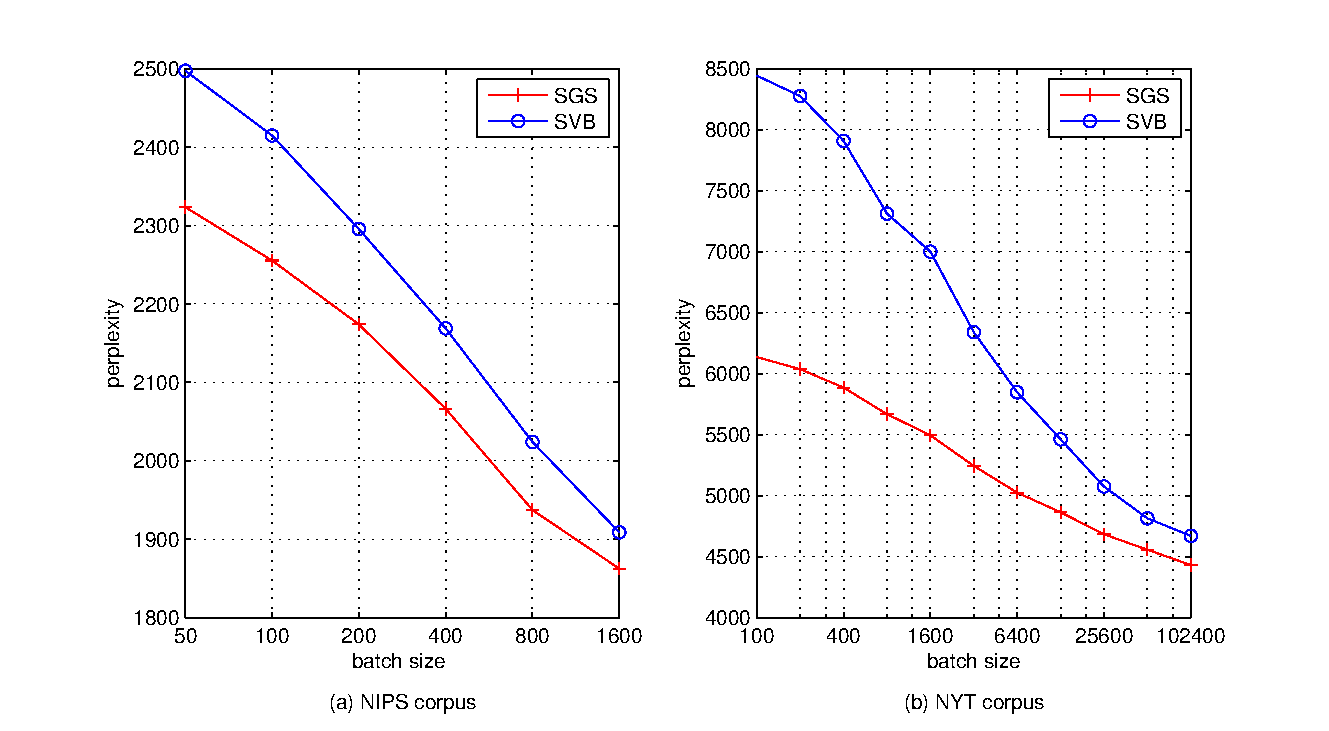
\includegraphics[width=\columnwidth*6/5]{pics/batch2.eps}}
%\caption{ Perplexities obtained by SVB and SGS on NIPS (left) and NYT (right)
%datasets for different mini-batch sizes. Specific parameter values are stated in text (\ref{sec:exp_setting}).
%The biggest mini-batch size for each plot is set as close to the dataset size as possible.}
%\label{fig:batch}
%\end{center}
%\vskip -0.2in
%\end{figure} 

\begin{figure}[ht]
\vskip 0.2in
\begin{center} 
\centering   
\subfigure[Perplexities of SVB and SGS on NIPS] 
{ \label{fig:batch_nips}
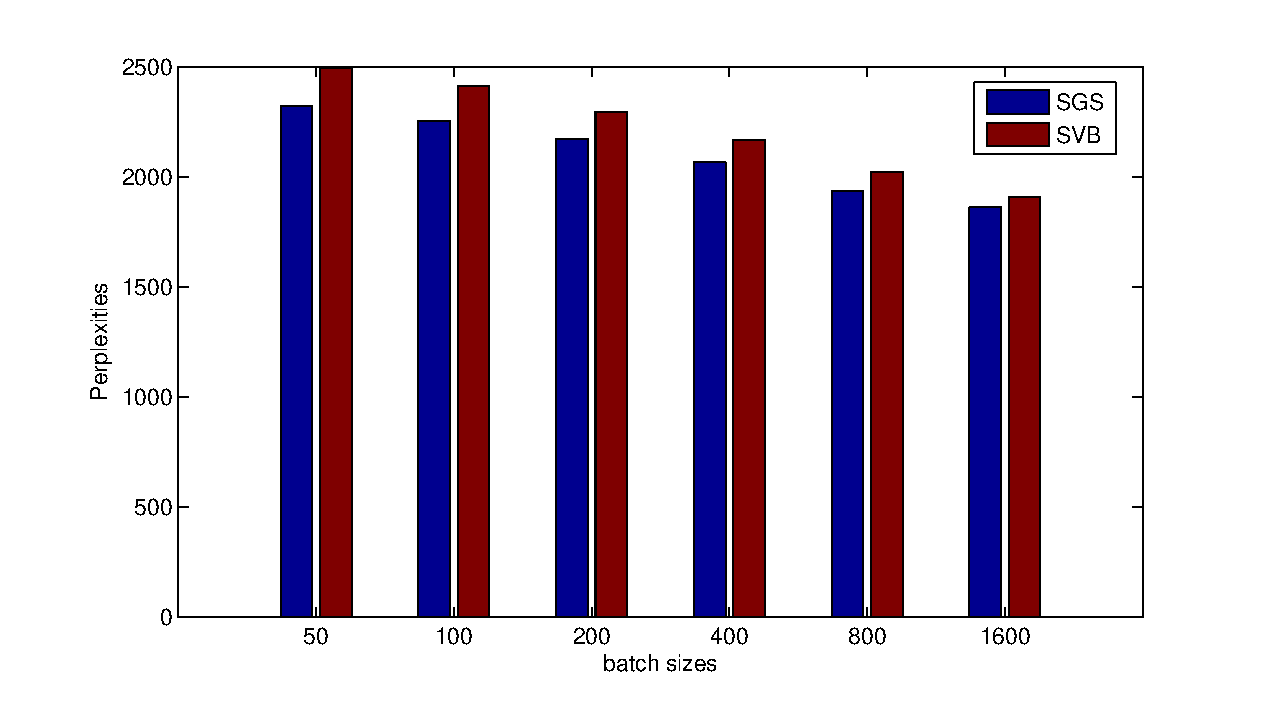
\includegraphics[width=\columnwidth]{pics/batch_NIPS.eps} 
}    
\subfigure[Perplexities of SVB and SGS on NYT] 
{ \label{fig:batch_nyt}    
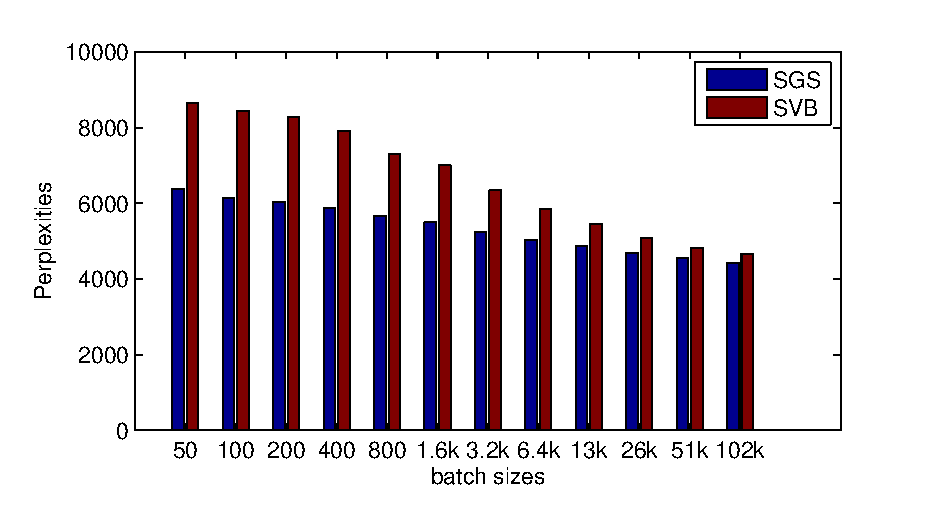
\includegraphics[width=\columnwidth]{pics/batch_NYT.eps}    
}    
\caption{ The perplexities obtained by SVB and SGS compared on a small (NIPS) and a large (NYT) dataset. One can conclude that SGS has moderate improvement over SVB in a dataset without much redundancy, while a huge improvement on the large one. The improvement is especially large when small batch sizes are used.}    
\label{fig:batch}    
\end{center}
\vskip -0.2in
\end{figure} 


\section{Experiments}
In this section, we would like to evaluate SGS's inference quality and computational efficiency. We're also interested in assessing how the parameters would affect SGS's performance, such as the hyper-parameter, the mini-batch size, the decay factor and the number of iterations. We will also give some intuitive examples which could shed light upon how SGS learns the knowledge.

We will demonstrate SGS using the SVB method \cite{broderick2013streaming} as the baseline. The latter one has been proved to have high inference quality that is similar to stochastic methods like SVI \cite{hoffman2013stochastic}. 

\subsection{Evaluation Method}
The predictive performance of LDA can be accessed by measuring the probability it has assigned to the holdout document. This metric is formalized by perplexity. First partition the dataset into 80 \% for training and the rest 20\% for testing. Let $\mathcal{M}$ denotes the model trained on the training data. Given a holdout document $d$, we can run the training procedure (with $\bm{\Phi}$ fixed) on the first half tokens of $d$ to get the document-topic distribution $\vec{\theta}_d$. Then calculate the exponentiated negative average of the log probability. Formally, given a trained model $\mathcal{M}$ and a holdout document $\vec{w}_{d}$, we have:
$$per(\vec{w}_{d}|\mathcal{M})=\exp-\frac{\sum_i \log p(w_{di}|\mathcal{M})}{|\vec{w}_{d}|}$$
where $\log p(w_{di}|\mathcal{M})=\sum_i \log {\sum_k \phi_{kw_{di}}\theta_{dk}}$. 

\subsection{Datasets}
To compare the performance of the algorithms in various setting, we test them on three datasets \footnote{All the three datasets can be downloaded from UCI Machine Learning Repository: \url{https://archive.ics.uci.edu/ml/datasets/Bag+of+Words}}. The small NIPS dataset \cite{pereiraeuclidean} has the articles from 1988 to 2000 that is accept by Neural Information Processing Systems (NIPS) Conferences. Each article has 1300 tokens on average, and the dataset has around 1740 articles, which gives us about 2 million tokens in total. Its dictionary has 13 thousand unique words. A larger dataset is the news from New York Times (NYT), which is composed of about 300 thousand documents and have around 100 million tokens altogether. There are about 100 thousand unique words in this corpus. And the largest one is the abstracts of the publications on PubMed, which contains around 8.2 million documents, with 730 million tokens in total\cite{UCI+Bache+Lichman:2013}. Because the baseline method SVB is slow to converge on the PubMed dataset, so we only perform analysis of SGS on PubMed, while comparing SGS against SVB in the NIPS and NYT datasets.

\label{sec:exp_setting}
In the following experiments, hyper-parameters $\alpha$ and $\beta$ are all set to $0.1$ and $0.03$ respectively. Without special remark, the SGS and SVB are both allowed to run until convergence. To be specific, the criterion for SGS is running Gibbs sampling for 400 iterations. For SVB, it's stop inner iteration if 1-norm of the change of $\theta_d$ divide the number of entries in $\theta_d$ is less than $0.00001$ or $100$ iterations; stop outer iteration if 1-norm of the change of $\phi$ divide the number of entries in $\phi$ is less than $0.001$. Further, the number of topics are set to $50$. 
 
\subsection{Results for various mini-batch size}
In this section, we test the two methods, SGS and SVB on both NIPS and NYT dataset, for various mini-batch sizes. To simplify our comparison, We simply set the decay factor for SGS as $\lambda=1$. Figure \ref{fig:batch}(a) and (b) show how two algorithms perform under this setting. In general, SGS performs consistently better than SVB, especially in the cases of bigger dataset and smaller mini-batch sizes. 

The different performance gap between SGS and SVB on NYT and NIPS dataset could be understood as different levels of redundancy. In order to be effective to learn in a streaming setting, it is required to have a redundant dataset. There are only 1740 documents in the NIPS corpus, which is far from being redundant and thus it's easy to imagine different streaming algorithms performs alike on this dataset. From the trend of the dataset size, we can expect that SGS would perform even better than SVB on larger datasets. Another interesting phenomenon is that SVB is more sensitive to batch size than SGS. SGS's ability to perform much better than SVB on smaller mini-batches have important advantages in practice.

In practical applications, online learning often faces a very large dataset. The number of rounds to process a new mini-batch is expected to be big enough to facilitate applications that need day-by-day update, for example, at least 100 rounds. Note that the second requirement is the basic difference between a batch algorithm and an online one. We argue that an experiment setting with less than 10 rounds shouldn't be considered as online. The NYT dataset with mini-batch size $3200$ is a typical case where people would encounter in practice. We can see that compared to the batch perplexity of $4300$, SGS obtains $5240$ while SVB reaches up to $6511$. SGS has great advantages over SVB in practical settings.

%TODO(this figure is not as perfect as possible, run the experiment for another 2 times) 
\begin{figure}[ht]
\vskip 0.2in
\begin{center}
\centerline{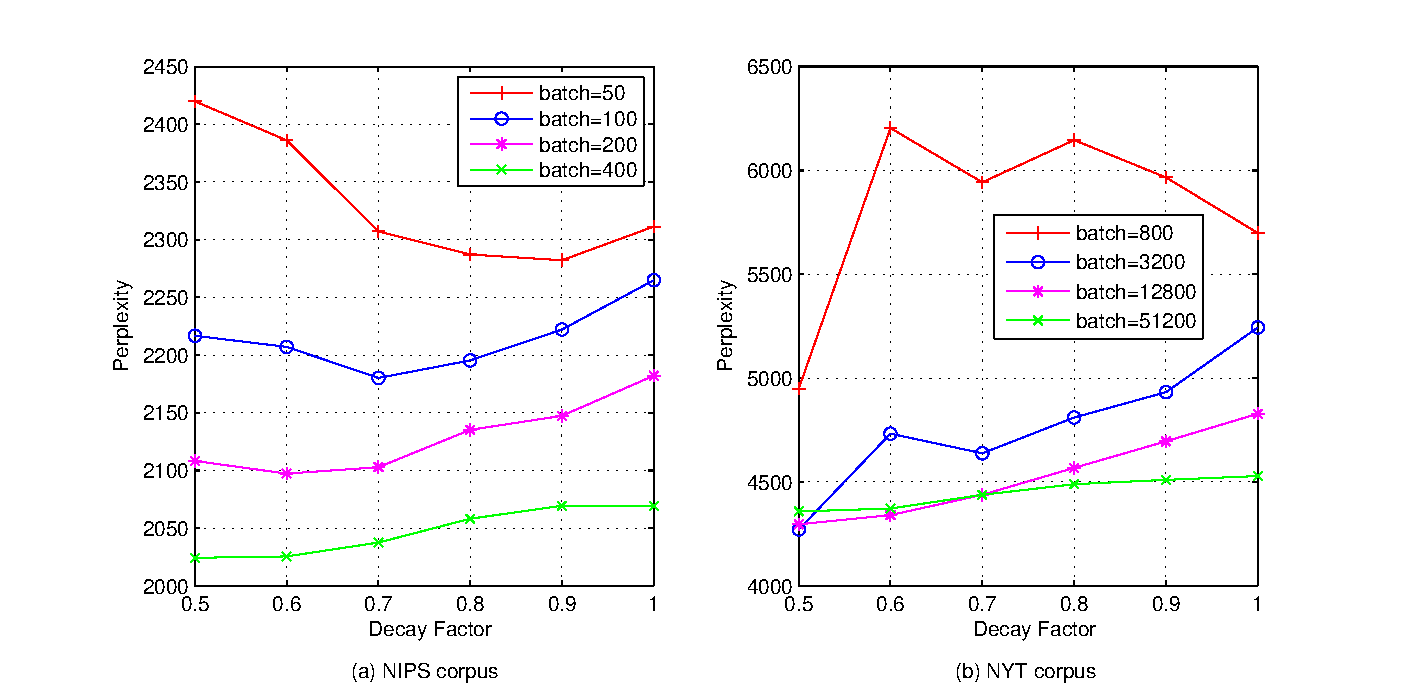
\includegraphics[width=\columnwidth*6/5]{pics/decay.eps}}
\caption{ On NIPS (left) and NYT (right) datasets, how decay factor $\lambda$ 
would affect SGS's performance. Parameters are set in the same way as it is claimed in Figure \ref{fig:batch}.}
\label{fig:decay}
\end{center}
\vskip -0.2in
\end{figure} 

%TODO(put simple introduction of SVB in the paper) 
\subsection{Results for different decay factor}
We also investigate how different decay factors $\lambda$ affect the performance of SGS under different dataset with a wide range of mini-batch sizes. The story is similar as above, bigger dataset has more obvious trends. As shown in Figure \ref{fig:decay}, when the mini-batch is too small, decay factor has a negative effect. It's probably because a small mini-batch could only learn limited knowledge in a round and its thus not preferable to forget the knowledge. When the mini-batch size is getting bigger, the decay factor will improve the performance, and the optimal value for $\lambda$ gets smaller as the batch size becomes larger. This could be reasoned with the same logic as the above, where bigger mini-batches will learn more and the next batch would have greater discrepancy with the current one. 

Let's reexamine the practical setting mentioned above, i.e. performance with batch size $3200$ on NYT dataset. We can see that a decay factor of $0.7$ could give a perplexity of $4640$, which is pretty close to the batch perplexity of $4300$. We have even observed that SGS could reach almost the same perplexity ($4350$) as batch algorithm with batch size $12800$ and decay factor $0.5$. We can conclude that, if the decay factor is set properly, SGS can almost reach the same precision as its batch counterpart in a practical setting (in this case, 100 rounds). 

\subsection{Learning Process}
\begin{figure}[ht]
\vskip 0.2in
\begin{center}
\centerline{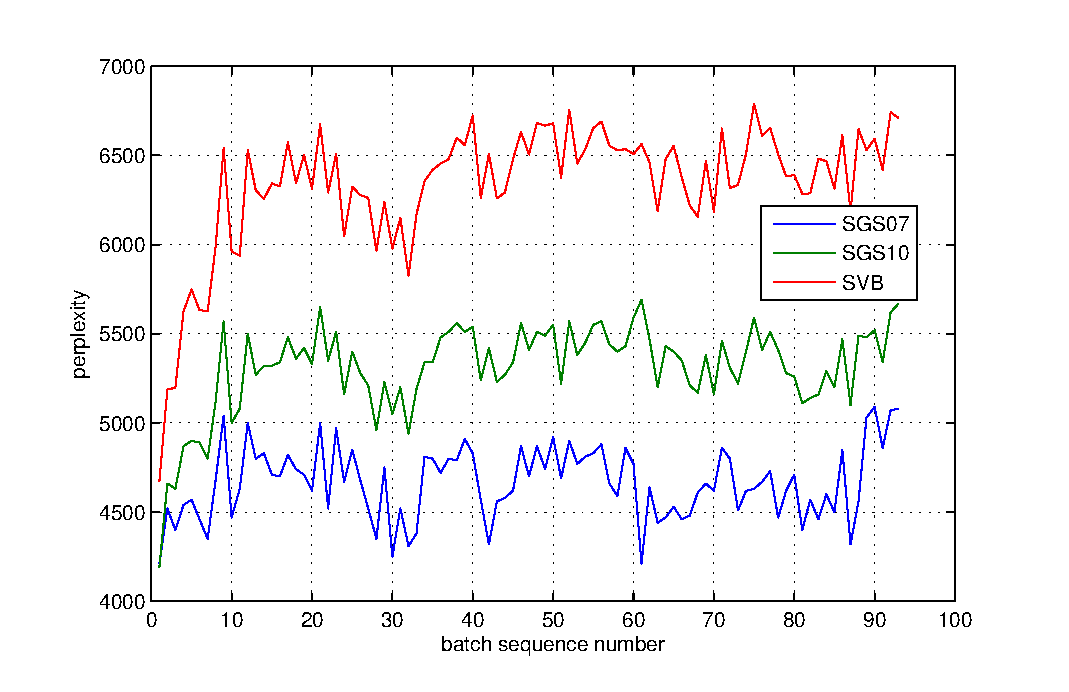
\includegraphics[width=\columnwidth]{pics/pro2.eps}}
\caption{The trend of changing perplexities as new mini-batches arrive. The 3 curves are acquired by running SVB, SGS(decay factor $1.0$) and SGS(decay factor $0.7$) on NYT dataset, with the typical application scenario of mini-batch size being $3200$. }
\label{fig:pro}
\end{center}
\vskip -0.2in
\end{figure} 
However, the mean perplexity of each mini-batch is not a full description of the learning process. We should also take the trend of the inference quality into account. In Figure \ref{fig:pro}, we plot the learning process of SVB and SGS (with different decay factors). We can clearly see that the performance of the decayed SGS is strictly better than the non-decayed version, and the latter one surpasses SVB. In other words, SGS can learn a better model as new data arrives. All three models have an initial perplexity bursts stage because the models have over-fitted the limited first few mini-batches. 

\subsection{Sample Topics}
To give the readers an intuition from a natural language perspective, we will show some topics here. To facilitate visualization purpose, we handicap both algorithms to discover only 10 topics on the NIPS dataset and thus we expected to see very general topics such as "neural network". We run SVB and SGS ($0.7$ decay) with the mini-batch size of $100$ until the $10$-th mini-batch (in the middle of a total of $16$ mini-batches), since we want to simulate the "anytime output" of an online algorithm. The most probable $5$ words in each topic are listed in Table \ref{tbl:sample_topics}, where the upper part outcome is from SVB while the lower part is from SGS.

The first 5 topics in SVB and the first 4 topics in SGS are about "neural networks". After a careful examination of how these topics are composed, we can conclude that SGS also outperforms SVB semantically. Even if the first 4 topics of SGS are all related to "neural network", they emphasize on various aspects, such as "analogy chip" or "control", and these emphasized views have high probabilities on the corresponding words. On the contrary, the "neural network" related topics output by SVB are mixed with each other. They assign high probabilities in general words, such as "learning", "network", and leaves the special words such as "control" with lower probability. 

\begin{table}[t]
\caption{The most probable $5$ words in each topic (ordered from the most probable to the least), output by SVB (upper) and SGS (lower) methods. They are the outputs after the $10$-th round learning on NIPS dataset, with a mini-batch size of $100$. Note that the topics are manually re-ordered, to make the "neural network" related topics on the top.}
\label{tbl:sample_topics}
\vskip 0.15in
\begin{center}
\begin{small}
%\begin{sc}
\begin{tabular}{llllll}
\hline
\abovespace\belowspace
{\sc Topic} & {\sc Keywords} \\
\hline
\abovespace
1 &  neural network model networks function \\
 2 & learning network time state control \\
 3 & learning network units hidden training \\
 4 & neurons synaptic input model neuron \\
 5 & memory network neural time input  \\
 6 & network data training set neural \\
 7 & visual model motion field figure \\
 8 & object features representation representations model\\
 9 & speech recognition neural input figure \\
 10 & model eye figure time phase\\
\hline
\hline
1 & network learning networks function information \\
2 & neuron neurons chip analog current\\
3 & output neural figure problem time \\
4 & control neural time model motor  \\
5 & image object figure images feature \\
6 & model space function results models \\
7 & training learning error hidden data \\
8 & model activity cells input time \\
9 & vector networks number neural data \\ 
10 & units unit representations set representation \\
\hline
\hline
\end{tabular}
%\end{sc}
\end{small}
\end{center}
\vskip -0.1in
\end{table}

\subsection{Evolution of topics}
To get a more intuitive understanding of what SGS and SVB have learned when new batches are processed, we show some examples on how topics are evolving during the learning process. With the NIPS dataset, we feed the documents chronologically into two algorithms. As above, we set the number of topics to $50$, mini-batch size to $100$ and the decay factor $\lambda$ of SGS to $0.7$. Due to the limit of space, we will only show the 'speech recognition' topic.

Table(\ref{tbl:evolution_of_topics}) has clearly shown the difference. SVB stuck to fix keywords from the $4$-th mini-batch, while SGS is adapting its topic-word distribution to fit the change. Moreover, SGS has shown the history of the research in speech recognition field. It starts from focusing on temporal signal, then the rising of HMM and finally HMM has dominating the field. On the other hand, the output of SVB don't have a single keyword of 'HMM' or 'context', which could possibly be explained as its incapability to adapt to newly generated keywords.

\begin{table}[t]
\caption{Evolution of topic 'speech recognition' chronologically output by SVB (upper) and SGS (lower). Each topic is represented by the most probable $7$ keywords.}
\label{tbl:evolution_of_topics}
\vskip 0.15in
\begin{center}
\begin{small}
%\begin{sc}
\begin{tabular}{llllll}
\hline
\abovespace\belowspace
{\sc Time} & {\sc Keywords} \\
\hline
\abovespace
1 & networks couplings local type dynamics phase complex \\
2 & speech recognition learning light networks phonetic  \\
3 & speech recognition networks learning synchrony light  \\
4 & speech recognition speaker networks phoneme experiments  \\
5 & speech recognition speaker networks phoneme phonetic  \\
6 & speech recognition speaker networks phoneme experiments  \\
7 & speech recognition speaker phoneme networks phonetic  \\
8-16 & speech recognition speaker phoneme networks experiments  \\

\hline
\hline
 1 & input temporal time signal rate fig patterns \\
 2 & input time temporal recognition speech signal patterns \\
 3 & recognition input speech time mlp temporal word \\
 4 & recognition speech input word time phoneme temporal \\
 5 & speech recognition word input time hmm speaker \\
 6 & recognition speech word input time hmm phoneme \\
 7 & word recognition speech input context hmm time \\
 8 & recognition word speech context input hmm time \\
 9 & speech word recognition hmm context input time \\
 10 & speech word recognition hmm context speaker input \\
 11-12 & speech word recognition hmm context input words \\
 13 & speech word recognition hmm context state words \\
 14 & speech word recognition hmm words context markov \\
 15 & speech word recognition hmm context words state \\
 16 & speech recognition hmm word state context hmms\\

\hline
\hline
\end{tabular}
%\end{sc}
\end{small}
\end{center}
\vskip -0.1in
\end{table}


\subsection{Distributed Experiments}
As topic model is widely used in the Internet industry, a scalable inference method should have the ability to efficiently and accurately process the huge amount of data generated every day. Thus, in this section we show the scalability of DSGS on the PubMed dataset. We've tested DSGS's performance with different batch sizes and parallel levels. In Figure(\ref{fig:dis_precision}), the distributed version has shown some interesting patterns in the precision of the inference. When the batch size is relatively big, such as 50k, the inference quality get worse as the number of threads going up, which conforms with the expectation. But things are going in the opposite direction when the batch size is small. The bigger level of the parallelism is, the better the performance is! This is consistent with some previous work in paralleling LDA \cite{broderick2013streaming}. On the other hand, the speed up is almost linear of the number of cores \ref{fig:dis_time}. Our distributed experiments is carried out in a 3 nodes, with a total of 36 cores cluster, which contains slow speed network data transmission. Due to the nature of the sparseness of topic-word assignments, SGS can take advantage of it and reduce the network bottleneck. In comparison, the parallel version of SVB contains dense update and hence doesn't fit well with large scale clusters.

%As shown in Figure(\ref{fig:dis_precision}), comparing to SGS, DSGS only suffer from a little performance loss. For example, with a moderate batch size of $3200$, SGS could achieve a perplexity of 4638, while DSGS with 8 threads is only slightly worse, 5102. However, the speed up is seven-fold, which is very useful in practice. Figure (\ref{fig:dis_time}) give us a sense of the timing result. We can see that DSGS could have nearly linear speed up.


\begin{figure}[ht]
\vskip 0.2in
\begin{center} 
\centering   
\subfigure[DSGS's experimental precision results on PubMed data, with various batch sizes and the number of threads. We can conclude that DSGS only suffer minor performance loss compared to the single thread version (SGS). The cluster has 3 nodes and each node is a 12-cores shared memory system.] 
{ \label{fig:dis_precision}
\includegraphics[width=\columnwidth]{pics/distributed_pubmed_pers.eps} 
}    
\subfigure[DSGS's time consumption under various number of threads as well as batch sizes. DSGS almost has linear acceleration on clusters.] 
{ \label{fig:dis_time}    
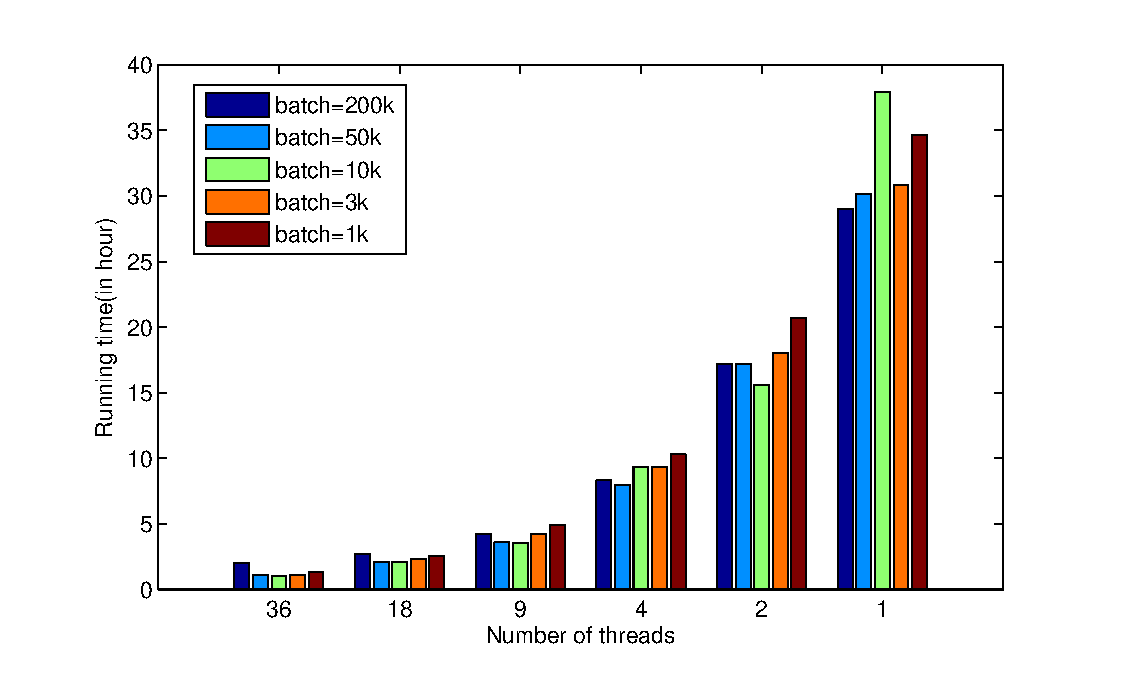
\includegraphics[width=\columnwidth]{pics/distributed_pubmed_times.eps}    
}    
\caption{ Distributed SGS's precision and efficiency. }    
\label{fig:dis}    
\end{center}
\vskip -0.2in
\end{figure} 

\section{Discussion}
We developed a streaming Gibbs sampling algorithm (SGS) for the LDA model. Our method can be seen as an online extension of the collapsed Gibbs sampling approach. The proposed method has theoretical root in Conditional Density Filtering (CDF). In theory, we have shown how SGS is improved over CDF-LDA. Moreover, our experimental results demonstrate that SGS improves perplexity over previous online methods, while maintaining similar computational burden. We have also shown that SGS could be well paralleled using similar techniques as those adopted in SVB. 

In the future, SGS can be further improved by making the decay factor $\lambda$, the batch size and the number of iteration for each document evolving, as more data feeds in. Intuitively, the algorithm learns fast at the beginning and later it slows down. Thus for example, it might be tempting to decrease the iteration count for each document to some constant over time. The scheme for the evolution deserves future research and it also needs strong theoretical guidance. 

% Acknowledgements should only appear in the accepted version. 
%\section*{Acknowledgments} 

\bibliography{example_paper}
\bibliographystyle{icml2015}

\end{document} 


% This document was modified from the file originally made available by
% Pat Langley and Andrea Danyluk for ICML-2K. This version was
% created by Lise Getoor and Tobias Scheffer, it was slightly modified  
% from the 2010 version by Thorsten Joachims & Johannes Fuernkranz, 
% slightly modified from the 2009 version by Kiri Wagstaff and 
% Sam Roweis's 2008 version, which is slightly modified from 
% Prasad Tadepalli's 2007 version which is a lightly 
% changed version of the previous year's version by Andrew Moore, 
% which was in turn edited from those of Kristian Kersting and 
% Codrina Lauth. Alex Smola contributed to the algorithmic style files.  
